\section{Benchmark stability}
\label{app:benchmark-stability}

This appendix reports the leave-one-dataset-out (LODO) configuration checks,
the mechanism-matched CIF check, and the method ordering by downstream learner,
value of $k$, and seed. All use the selected configurations of the main
benchmark.

\subsection{LODO configuration sensitivity}

Each LODO run selects configurations on all but one dataset of the panel,
scores the held-out dataset, and averages scores and ranks over downstream
learners and standard values of $k$.
\Cref{tab:lodo-config-sensitivity,tab:lodo-config-sensitivity-allmethod} report
the complete-case and all-method panels. Every single-configuration family
keeps its held-out score exactly, which checks the reselection code. Its mean
rank moves only as the tuned families are reselected around it, by at most 0.05
in classification and 0.125 in regression. On the all-method panels CIF loses
0.002 balanced accuracy and 0.008 $R^2$ under reselection, and XGBoost loses
0.03 $R^2$ (0.270 against 0.241). The one large reselection effect is cforest
in regression, whose alternative configuration is chosen on one holdout and
scores far lower there (mean $R^2$ 0.30 against 0.20).

\begin{table}[!htbp]
  \centering
  \fontsize{8}{9.1}\selectfont
  \setlength{\tabcolsep}{2.5pt}
  \renewcommand{\arraystretch}{1.0}
  \begin{tabular*}{\linewidth}{@{\extracolsep{\fill}}l
    S[table-format=2.2]
    S[table-format=2.2]
    S[table-format=1.3]
    S[table-format=1.0]
    c
    @{\hspace{0.8em}}
    l
    S[table-format=2.2]
    S[table-format=2.2]
    S[table-format=-1.3]
    S[table-format=1.0]
    c@{}}
    \toprule
    \multicolumn{6}{c}{Classification} &
    \multicolumn{6}{c}{Regression} \\
    \cmidrule(lr){1-6}\cmidrule(l){7-12}
    \tablehead{Method} & {LODO} & {Fixed} & {Score} & {Settings} & {Main} &
    \tablehead{Method} & {LODO} & {Fixed} & {Score} & {Settings} & {Main} \\
    \midrule
    RF-RFE & 2.54 & 2.54 & 0.825 & 1 & \countfrac{13}{13} & ExtraTrees & 4.67 & 4.67 & 0.292 & 1 & \countfrac{6}{6} \\
    LightGBM & 4.31 & 4.46 & 0.813 & 1 & \countfrac{13}{13} & CatBoost & 6.17 & 6.33 & 0.229 & 1 & \countfrac{6}{6} \\
    RF & 5.08 & 5.23 & 0.802 & 1 & \countfrac{13}{13} & RF-RFE & 6.67 & 6.67 & 0.333 & 1 & \countfrac{6}{6} \\
    CatBoost & 5.54 & 5.69 & 0.801 & 1 & \countfrac{13}{13} & RF & 6.83 & 7.00 & 0.260 & 1 & \countfrac{6}{6} \\
    XGBoost & 5.69 & 4.92 & 0.808 & 2 & \countfrac{11}{13} & RT & 7.00 & 7.00 & 0.266 & 1 & \countfrac{6}{6} \\
    Boruta & 6.23 & 6.38 & 0.791 & 1 & \countfrac{13}{13} & CIF & 7.33 & 7.00 & 0.240 & 2 & \countfrac{4}{6} \\
    ExtraTrees & 6.62 & 6.77 & 0.792 & 1 & \countfrac{13}{13} & XGBoost & 8.50 & 8.67 & 0.149 & 2 & \countfrac{5}{6} \\
    CIF & 6.85 & 6.38 & 0.793 & 2 & \countfrac{11}{13} & DT & 8.67 & 8.83 & 0.124 & 1 & \countfrac{6}{6} \\
    cforest & 8.23 & 8.46 & 0.785 & 1 & \countfrac{13}{13} & Boruta & 9.17 & 9.33 & 0.118 & 1 & \countfrac{6}{6} \\
    DT & 9.38 & 9.46 & 0.763 & 1 & \countfrac{13}{13} & LightGBM & 10.50 & 10.50 & -0.214 & 1 & \countfrac{6}{6} \\
    RDC filter & 10.69 & 10.85 & 0.764 & 1 & \countfrac{13}{13} & CIT & 10.67 & 10.50 & -0.206 & 2 & \countfrac{5}{6} \\
    ctree & 11.77 & 11.77 & 0.749 & 1 & \countfrac{13}{13} & cforest & 10.67 & 9.67 & 0.092 & 2 & \countfrac{5}{6} \\
    CIT & 12.15 & 12.15 & 0.754 & 1 & \countfrac{13}{13} & PI & 11.00 & 11.00 & -0.024 & 1 & \countfrac{6}{6} \\
    MC filter & 12.69 & 12.69 & 0.737 & 1 & \countfrac{13}{13} & ctree & 11.33 & 11.50 & 0.051 & 1 & \countfrac{6}{6} \\
    RT & 13.00 & 13.00 & 0.737 & 1 & \countfrac{13}{13} & PC filter & 11.67 & 11.83 & 0.099 & 1 & \countfrac{6}{6} \\
    PI & 15.73 & 15.73 & 0.676 & 1 & \countfrac{13}{13} & RDC filter & 12.50 & 12.67 & -0.082 & 1 & \countfrac{6}{6} \\
    CPI & 16.50 & 16.50 & 0.600 & 1 & \countfrac{13}{13} & DC filter & 13.50 & 13.67 & -0.009 & 1 & \countfrac{6}{6} \\
    \multicolumn{6}{c}{} & CPI & 14.17 & 14.17 & -0.554 & 1 & \countfrac{6}{6} \\
    \bottomrule
  \end{tabular*}
  \caption{LODO configuration sensitivity on the complete-case panels (13
  classification and 6 regression datasets). LODO is the mean rank when each
  held-out dataset is scored with configurations selected on the other
  datasets; Fixed is the mean rank on the same panel under the configuration
  selected on the full benchmark. Lower rank is better; rows are ordered by LODO
  rank within each task. Score is the mean held-out metric under LODO
  selection. Settings reports the number of distinct selected configurations;
  Main reports how often the main benchmark configuration is reselected. Ranks
  are computed within held-out datasets before averaging, so score order need
  not match rank order. Entries are mean ranks over the panel datasets; the difference between the fixed and LODO columns is the reported sensitivity.}
  \label{tab:lodo-config-sensitivity}
\end{table}

\begin{table}[!htbp]
  \centering
  \fontsize{8}{9.1}\selectfont
  \setlength{\tabcolsep}{2.5pt}
  \renewcommand{\arraystretch}{1.0}
  \begin{tabular*}{\linewidth}{@{\extracolsep{\fill}}l
    S[table-format=2.2]
    S[table-format=2.2]
    S[table-format=1.3]
    S[table-format=1.0]
    c
    @{\hspace{0.8em}}
    l
    S[table-format=2.2]
    S[table-format=2.2]
    S[table-format=-1.3]
    S[table-format=1.0]
    c@{}}
    \toprule
    \multicolumn{6}{c}{Classification} &
    \multicolumn{6}{c}{Regression} \\
    \cmidrule(lr){1-6}\cmidrule(l){7-12}
    \tablehead{Method} & {LODO} & {Fixed} & {Score} & {Settings} & {Main} &
    \tablehead{Method} & {LODO} & {Fixed} & {Score} & {Settings} & {Main} \\
    \midrule
    RF-RFE & 4.19 & 4.19 & 0.837 & 1 & \countfrac{21}{21} & ExtraTrees & 5.00 & 5.00 & 0.353 & 1 & \countfrac{8}{8} \\
    XGBoost & 5.81 & 5.81 & 0.828 & 1 & \countfrac{21}{21} & CIF & 6.50 & 6.25 & 0.315 & 2 & \countfrac{7}{8} \\
    RF & 5.86 & 5.86 & 0.823 & 1 & \countfrac{21}{21} & CatBoost & 6.62 & 6.75 & 0.304 & 1 & \countfrac{8}{8} \\
    LightGBM & 6.05 & 6.05 & 0.829 & 1 & \countfrac{21}{21} & RF-RFE & 6.88 & 6.88 & 0.382 & 1 & \countfrac{8}{8} \\
    CIF & 6.10 & 5.86 & 0.820 & 2 & \countfrac{20}{21} & RF & 7.50 & 7.63 & 0.327 & 1 & \countfrac{8}{8} \\
    Boruta & 6.57 & 6.62 & 0.816 & 1 & \countfrac{21}{21} & RT & 8.25 & 8.25 & 0.330 & 1 & \countfrac{8}{8} \\
    CatBoost & 6.71 & 6.76 & 0.822 & 1 & \countfrac{21}{21} & DT & 9.25 & 9.38 & 0.225 & 1 & \countfrac{8}{8} \\
    ExtraTrees & 7.29 & 7.33 & 0.817 & 1 & \countfrac{21}{21} & Boruta & 9.38 & 9.50 & 0.221 & 1 & \countfrac{8}{8} \\
    cforest & 8.29 & 8.33 & 0.812 & 1 & \countfrac{21}{21} & cforest & 9.50 & 8.75 & 0.202 & 2 & \countfrac{7}{8} \\
    DT & 8.62 & 8.62 & 0.799 & 1 & \countfrac{21}{21} & PC filter & 9.75 & 9.88 & 0.207 & 1 & \countfrac{8}{8} \\
    RDC filter & 11.00 & 11.05 & 0.794 & 1 & \countfrac{21}{21} & XGBoost & 10.00 & 10.13 & 0.241 & 2 & \countfrac{7}{8} \\
    PI & 11.67 & 11.67 & 0.745 & 1 & \countfrac{21}{21} & LightGBM & 10.12 & 10.13 & -0.028 & 1 & \countfrac{8}{8} \\
    MC filter & 11.86 & 11.86 & 0.778 & 1 & \countfrac{21}{21} & RDC filter & 10.88 & 11.00 & 0.071 & 1 & \countfrac{8}{8} \\
    RT & 12.81 & 12.81 & 0.780 & 1 & \countfrac{21}{21} & CIT & 11.25 & 11.13 & -0.023 & 2 & \countfrac{7}{8} \\
    ctree & 12.86 & 12.86 & 0.785 & 1 & \countfrac{21}{21} & ctree & 11.25 & 11.38 & 0.167 & 1 & \countfrac{8}{8} \\
    CIT & 13.14 & 13.14 & 0.788 & 1 & \countfrac{21}{21} & PI & 11.75 & 11.75 & 0.112 & 1 & \countfrac{8}{8} \\
    CPI & 14.19 & 14.19 & 0.694 & 1 & \countfrac{21}{21} & DC filter & 12.12 & 12.25 & 0.126 & 1 & \countfrac{8}{8} \\
    \multicolumn{6}{c}{} & CPI & 15.00 & 15.00 & -0.292 & 1 & \countfrac{8}{8} \\
    \bottomrule
  \end{tabular*}
  \caption{LODO configuration sensitivity on the all-method panels (21 classification and 8 regression datasets) used by the main table. Columns as in \cref{tab:lodo-config-sensitivity}; the Fixed column repeats the main-table mean ranks.}
  \label{tab:lodo-config-sensitivity-allmethod}
\end{table}

\subsection{Mechanism-matched CIF check}
\label{app:cif-perm-check}

The benchmark ranks cforest by partykit's out-of-bag permutation importance and
CIF by split importance, so the margin between them mixes the importance
mechanism with the way the trees are grown. To separate the two, the selected
CIF configuration of each task was refit on every training fold of 20
classification and 8 regression datasets and ranked by the cforest mechanism:
one permutation of each feature on each tree's out-of-bag rows, with the error
increase averaged over the 100 trees. The rankings were scored with the
benchmark protocol. The 20 classification datasets are the 22 on which CIF and
cforest are paired, less \nolinkurl{gisette} and \nolinkurl{letter}, which were not refit.

\Cref{tab:cif-perm-check} gives the result. In classification the margin over
cforest is unchanged, so it persists under a common importance mechanism. In
regression the medians agree ($+0.006$ over cforest, $-0.002$ against
split-ranked CIF), and the negative means come from one dataset, coepra2
($n=76$, 5,144 predictors), on which every method has negative $R^2$. The
conclusion is therefore stated for classification.

Permutation importance computed on the training rows scores well below both
rankings. On the 16 classification datasets that completed, it scores 0.10 below cforest
and 0.12 below split-ranked CIF, with the loss concentrated on the small-$n$,
high-$p$ datasets. On the high-$p$ datasets the refit's split ranking also
overlaps the stored benchmark ranking poorly in the top ten (mean Jaccard 0.38
in classification), because most features never split there and their tied
zero importances fall in arbitrary order. On the low-$p$ datasets the overlap
is complete.

\begin{table}[!htbp]
  \centering
  \footnotesize
  \setlength{\tabcolsep}{5pt}
  \begin{tabular}{@{}lrrrc@{}}
    \toprule
    \tablehead{Comparison} & Datasets & Mean & Median & Wins--losses \\
    \midrule
    \multicolumn{5}{@{}l}{\emph{Classification (balanced accuracy)}} \\
    CIF (out-of-bag permutation) vs cforest & 20 & +0.012 & +0.006 & \winloss{15}{5} \\
    CIF (out-of-bag permutation) vs CIF (split) & 20 & +0.001 & $-$0.001 & \winloss{8}{12} \\
    CIF (split) vs cforest & 20 & +0.011 & +0.008 & \winloss{16}{4} \\
    CIF (training-row permutation) vs cforest & 16 & $-$0.100 & $-$0.055 & \winloss{6}{10} \\
    \addlinespace
    \multicolumn{5}{@{}l}{\emph{Regression ($R^2$)}} \\
    CIF (out-of-bag permutation) vs cforest & 8 & $-$0.115 & +0.006 & \winloss{6}{2} \\
    CIF (out-of-bag permutation) vs CIF (split) & 8 & $-$0.136 & $-$0.002 & \winloss{4}{4} \\
    CIF (split) vs cforest & 8 & +0.021 & +0.009 & \winloss{6}{2} \\
    CIF (training-row permutation) vs cforest & 6 & $-$0.016 & +0.006 & \winloss{4}{2} \\
    \bottomrule
  \end{tabular}
  \caption{CIF ranked by the importance mechanism of cforest. Directed differences in dataset-mean score (balanced accuracy or $R^2$ over downstream learners and standard $k$) between the first and second method, summarized over datasets: mean, median, and the number of datasets on which the first method scores higher or lower. Out-of-bag permutation is partykit-style out-of-bag permutation importance computed on the refit CIF; training-row permutation is scikit-learn permutation importance on the training rows (16 and 6 datasets completed). The pendigits dataset enters the out-of-bag rows with four of its five seeds.}
  \label{tab:cif-perm-check}
\end{table}

\subsection{Breakdowns by downstream learner, \texorpdfstring{top-$k$}{top-k} value, and seed}

The main benchmark averages over downstream learners, standard values of $k$,
folds, and seeds. The next tables show how method ordering changes when results
are split by downstream learner, value of $k$, and seed. They use the
same selected method configurations as the main benchmark.

For the learner and $k$ checks, one unit is one downstream learner paired with
one standard value of $k$. Within each unit, methods are ordered by mean rank
among datasets where every benchmark method is available for that learner-by-$k$
combination; ties use average ranks.
\Cref{tab:classification-learner-k-sensitivity,tab:regression-learner-k-sensitivity}
show all 15 learner-by-$k$ combinations for each task. Rows follow the main
benchmark order. The
learner columns report mean position over the five standard values of $k$ for
that learner; lower positions are better. Mean position averages the positions
obtained after ordering methods within each learner-by-$k$ combination; mean
rank averages the dataset-level ranks directly. Top 3 of 15 and Top 5 of 15
count the learner-by-$k$ combinations where the method ranks in the top 3 or
top 5.

\begin{table}[!htbp]
  \centering
  \footnotesize
  \setlength{\tabcolsep}{3pt}
  \renewcommand{\arraystretch}{1.04}
  \begin{tabular}{@{}l
    S[table-format=2.1]
    S[table-format=2.1]
    S[table-format=2.1]
    S[table-format=2.1]
    S[table-format=2.1]
    c
    c
    c@{}}
    \toprule
    \tablehead{Method} & {KNN} & {LR} & {SVM} & {Mean position} & {Mean rank} & {Best/worst} &
    \shortstack{Top 3\\of 15} & \shortstack{Top 5\\of 15} \\
    \midrule
    RF-RFE & 1.7 & 5.0 & 1.8 & 2.8 & 5.2 & 1.0/8.0 & \countfrac{10}{15} & \countfrac{13}{15} \\
    XGBoost & 5.4 & 2.7 & 3.4 & 3.8 & 5.8 & 2.0/8.0 & \countfrac{9}{15} & \countfrac{11}{15} \\
    CIF & 4.2 & 4.4 & 5.7 & 4.8 & 6.7 & 2.0/7.0 & \countfrac{3}{15} & \countfrac{10}{15} \\
    RF & 3.6 & 5.1 & 5.1 & 4.6 & 6.4 & 1.5/7.0 & \countfrac{3}{15} & \countfrac{10}{15} \\
    LightGBM & 4.2 & 2.2 & 2.0 & 2.8 & 5.5 & 1.0/6.0 & \countfrac{11}{15} & \countfrac{13}{15} \\
    Boruta & 5.2 & 8.6 & 7.8 & 7.2 & 7.5 & 1.0/9.0 & \countfrac{2}{15} & \countfrac{2}{15} \\
    CatBoost & 6.1 & 3.4 & 4.1 & 4.5 & 6.3 & 1.0/8.0 & \countfrac{5}{15} & \countfrac{10}{15} \\
    ExtraTrees & 6.8 & 7.6 & 8.8 & 7.7 & 7.7 & 2.0/12.0 & \countfrac{1}{15} & \countfrac{1}{15} \\
    cforest & 9.5 & 7.6 & 9.3 & 8.8 & 8.2 & 5.0/11.0 & \countfrac{0}{15} & \countfrac{1}{15} \\
    DT & 10.4 & 9.2 & 8.4 & 9.3 & 9.5 & 4.0/13.5 & \countfrac{0}{15} & \countfrac{2}{15} \\
    RDC filter & 11.2 & 12.0 & 12.6 & 11.9 & 10.8 & 10.0/15.0 & \countfrac{0}{15} & \countfrac{0}{15} \\
    PI & 15.3 & 15.8 & 15.8 & 15.6 & 13.4 & 13.5/16.0 & \countfrac{0}{15} & \countfrac{0}{15} \\
    MC filter & 12.0 & 13.6 & 13.8 & 13.1 & 11.3 & 10.0/17.0 & \countfrac{0}{15} & \countfrac{0}{15} \\
    RT & 15.0 & 13.0 & 13.5 & 13.8 & 11.9 & 10.0/16.0 & \countfrac{0}{15} & \countfrac{0}{15} \\
    ctree & 12.1 & 13.0 & 12.4 & 12.5 & 11.0 & 10.0/15.0 & \countfrac{0}{15} & \countfrac{0}{15} \\
    CIT & 13.3 & 12.8 & 11.7 & 12.6 & 11.0 & 9.0/16.0 & \countfrac{0}{15} & \countfrac{0}{15} \\
    CPI & 17.0 & 17.0 & 16.8 & 16.9 & 14.8 & 16.0/17.0 & \countfrac{0}{15} & \countfrac{0}{15} \\
    \bottomrule
  \end{tabular}
  \caption{Classification sensitivity by downstream learner and value of $k$.
  Lower values are better. KNN, LR, and SVM denote downstream learners;
  Top 3 of 15 and Top 5 of 15 count the learner-by-$k$ combinations where the
  method ranks in the top 3 or top 5. The learner columns and mean position
  average the method's ordinal position among the methods over learner-by-$k$
  combinations (the five values of $k$ for one learner, or all 15 combinations);
  best and worst are its extreme positions over the 15 combinations; mean rank
  averages its dataset-level rank over datasets and combinations. The dataset
  counts at $k=5,10,25,50,100$ are 21, 20, 14, 14, and 13. The spread across learner and $k$ columns is the reported sensitivity.}
  \label{tab:classification-learner-k-sensitivity}
\end{table}

In the classification learner-by-$k$ sensitivity table, CIF is top five in 10 of
the 15 learner-by-$k$ combinations and top three in 3 of 15. Its mean position
is close to RF's and is better than the single-tree and filter baselines in the
mean-position summary. RF-RFE, LightGBM, XGBoost, and CatBoost have lower mean
positions.

\begin{table}[!htbp]
  \centering
  \footnotesize
  \setlength{\tabcolsep}{3pt}
  \renewcommand{\arraystretch}{1.04}
  \begin{tabular}{@{}l
    S[table-format=2.1]
    S[table-format=2.1]
    S[table-format=2.1]
    S[table-format=2.1]
    S[table-format=2.1]
    c
    c
    c@{}}
    \toprule
    \tablehead{Method} & {KNN} & {Ridge} & {SVR} & {Mean position} & {Mean rank} & {Best/worst} &
    \shortstack{Top 3\\of 15} & \shortstack{Top 5\\of 15} \\
    \midrule
    ExtraTrees & 6.2 & 2.4 & 2.6 & 3.7 & 6.8 & 1.0/11.0 & \countfrac{9}{15} & \countfrac{11}{15} \\
    CIF & 4.6 & 9.9 & 2.4 & 5.6 & 7.8 & 1.0/12.0 & \countfrac{7}{15} & \countfrac{8}{15} \\
    CatBoost & 2.0 & 8.9 & 3.2 & 4.7 & 7.3 & 1.0/15.0 & \countfrac{6}{15} & \countfrac{12}{15} \\
    RF-RFE & 3.2 & 3.0 & 5.9 & 4.0 & 7.1 & 1.0/9.0 & \countfrac{7}{15} & \countfrac{11}{15} \\
    RF & 7.8 & 4.2 & 10.0 & 7.3 & 8.3 & 2.0/13.0 & \countfrac{2}{15} & \countfrac{4}{15} \\
    RT & 4.4 & 10.0 & 6.1 & 6.8 & 8.5 & 2.0/17.0 & \countfrac{3}{15} & \countfrac{7}{15} \\
    cforest & 11.4 & 11.7 & 9.9 & 11.0 & 10.1 & 6.0/16.0 & \countfrac{0}{15} & \countfrac{0}{15} \\
    DT & 6.7 & 9.4 & 9.1 & 8.4 & 9.0 & 4.0/16.0 & \countfrac{0}{15} & \countfrac{2}{15} \\
    Boruta & 12.5 & 4.4 & 11.9 & 9.6 & 9.4 & 2.0/16.0 & \countfrac{2}{15} & \countfrac{2}{15} \\
    PC filter & 12.8 & 12.0 & 11.0 & 11.9 & 10.7 & 8.0/16.0 & \countfrac{0}{15} & \countfrac{0}{15} \\
    LightGBM & 9.2 & 10.4 & 9.8 & 9.8 & 9.6 & 1.0/17.0 & \countfrac{3}{15} & \countfrac{3}{15} \\
    XGBoost & 6.5 & 15.9 & 9.3 & 10.6 & 9.9 & 1.5/18.0 & \countfrac{1}{15} & \countfrac{4}{15} \\
    RDC filter & 14.3 & 10.1 & 6.5 & 10.3 & 9.8 & 3.0/16.0 & \countfrac{1}{15} & \countfrac{2}{15} \\
    CIT & 14.7 & 12.4 & 14.7 & 13.9 & 11.0 & 8.5/18.0 & \countfrac{0}{15} & \countfrac{0}{15} \\
    ctree & 8.2 & 9.2 & 17.4 & 11.6 & 10.9 & 1.0/18.0 & \countfrac{2}{15} & \countfrac{4}{15} \\
    PI & 12.3 & 7.1 & 14.4 & 11.3 & 10.2 & 3.0/16.0 & \countfrac{1}{15} & \countfrac{2}{15} \\
    DC filter & 16.4 & 13.9 & 9.6 & 13.3 & 11.1 & 7.0/17.0 & \countfrac{0}{15} & \countfrac{0}{15} \\
    CPI & 17.8 & 16.1 & 17.2 & 17.0 & 13.6 & 9.5/18.0 & \countfrac{0}{15} & \countfrac{0}{15} \\
    \bottomrule
  \end{tabular}
  \caption{Regression sensitivity by downstream learner and value of $k$.
  Lower values are better. KNN, Ridge, and SVR denote downstream
  learners; Top 3 of 15 and Top 5 of 15 count the learner-by-$k$ combinations
  where the method ranks in the top 3 or top 5. The learner columns and mean
  position average the method's ordinal position among the methods over
  learner-by-$k$ combinations (the five values of $k$ for one learner, or all 15
  combinations); best and worst are its extreme positions over the 15
  combinations; mean rank averages its dataset-level rank over datasets and
  combinations. The dataset counts at $k=5,10,25,50,100$ are 8, 8, 7, 7, and 6.
  The spread across learner and $k$ columns is the reported sensitivity.}
  \label{tab:regression-learner-k-sensitivity}
\end{table}

CIF has the fourth-lowest regression mean position in this breakdown, after
ExtraTrees, RF-RFE, and CatBoost, and remains ahead of ctree, cforest, CIT, and
most filter and wrapper methods in this summary. The pairwise figures use the
datasets available for each comparator.

\begin{figure}[!htbp]
  \centering
  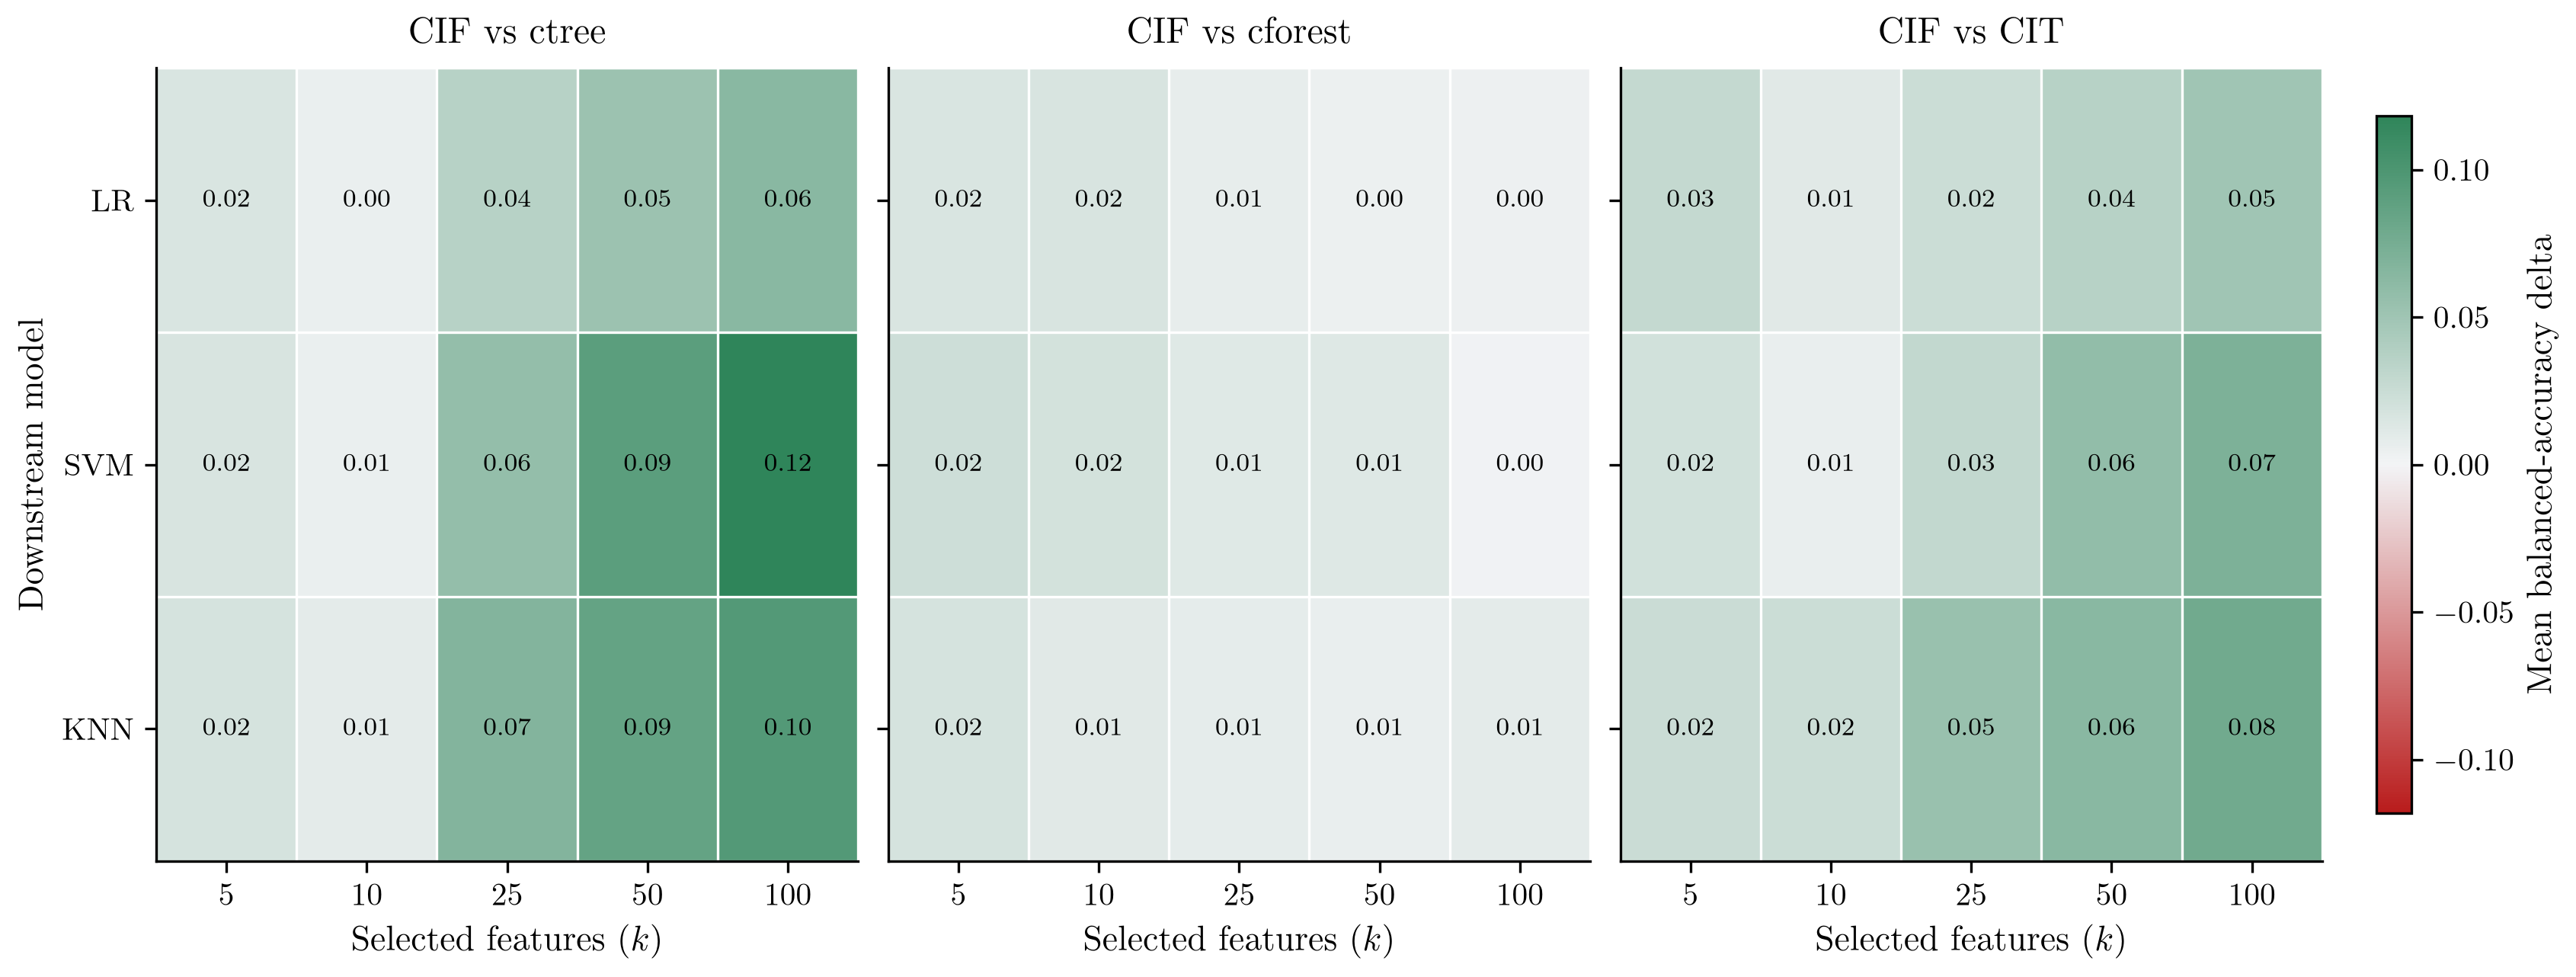
\includegraphics[width=0.88\linewidth]{figures/benchmark_pairwise_sensitivity.png}
  \caption{Classification CIF margins against ctree, cforest, and CIT by
  downstream learner and value of $k$. Each plotted value is the
  mean balanced-accuracy difference, CIF minus comparator, for one
  downstream learner and one value of $k$; positive values favor CIF. Dataset
  counts by $k$ are 21, 20, 14, 14, and 13 for ctree, 22, 21, 15, 15, and 14
  for cforest, and 23, 22, 16, 16, and 15 for CIT. Values are means over datasets; the bootstrap intervals for the pooled differences are in \cref{tab:conditional-inference-comparisons}.}
  \label{fig:benchmark-pairwise-sensitivity}
\end{figure}

\begin{figure}[!htbp]
  \centering
  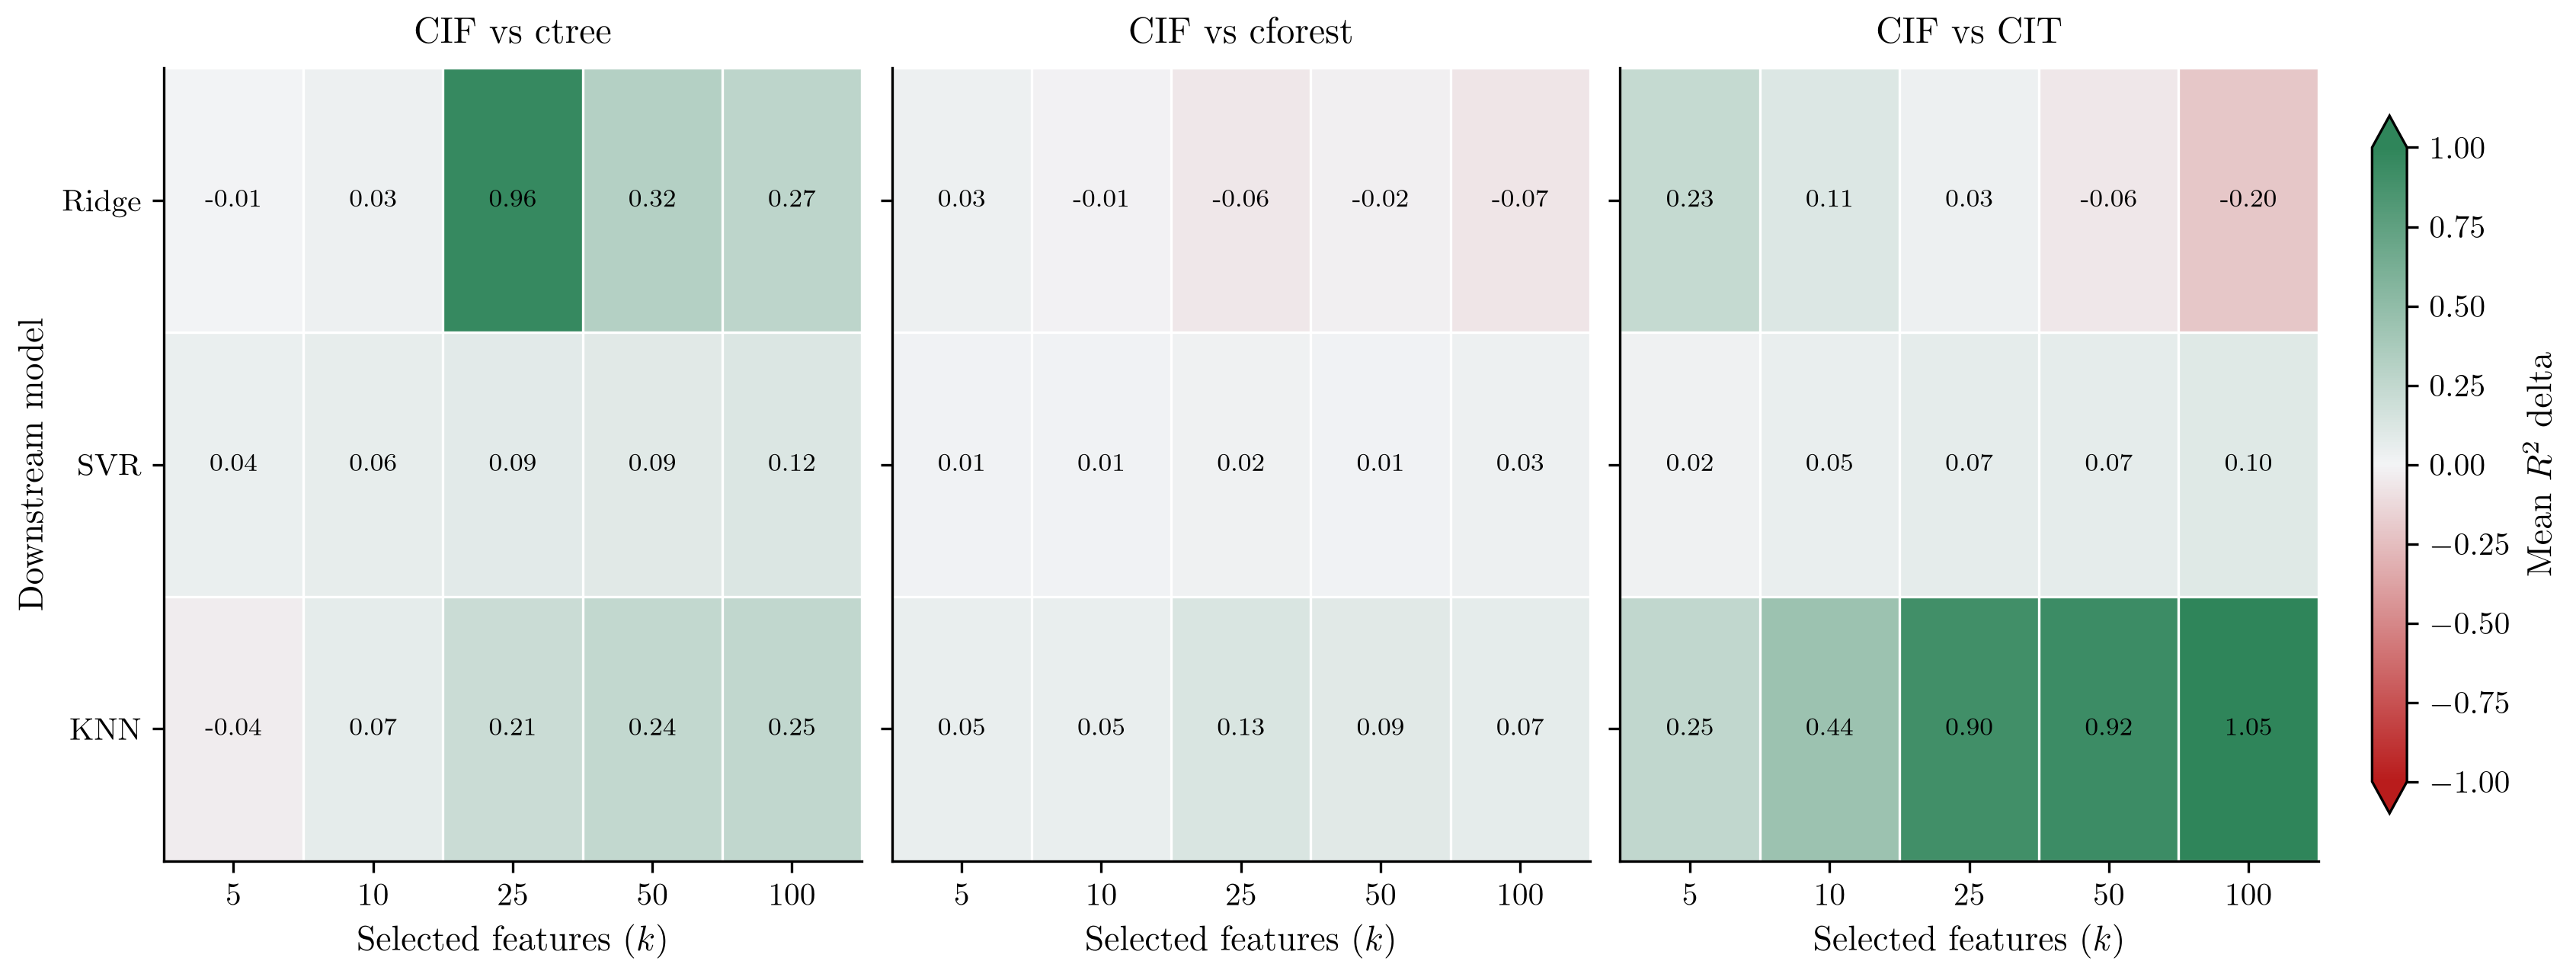
\includegraphics[width=0.88\linewidth]{figures/regression_benchmark_pairwise_sensitivity.png}
  \caption{Regression CIF margins against ctree, cforest, and CIT by
  downstream learner and value of $k$. Each plotted value is the mean
  $R^2$ difference, CIF minus comparator, for one downstream
  learner and one value of $k$; positive values favor CIF. Dataset counts by
  $k$ are 8, 8, 7, 7, and 6 for each comparison. Large positive plotted values
  can reflect negative mean $R^2$ for the comparator. Numeric labels show the
  unclipped values; the color scale is clipped at $\pm1$ for readability. Values are means over datasets; the bootstrap intervals for the pooled differences are in \cref{tab:conditional-inference-comparisons}.}
  \label{fig:regression-benchmark-pairwise-sensitivity}
\end{figure}

For the seed checks, each method is ranked separately within each fixed seed.
Keeping only datasets with results for every method, downstream learner,
standard top-$k$ value, and seed leaves 13 classification datasets and 6
regression datasets complete across all five seeds. These tables summarize seed
variation by rank without intervals or tests. In these tables, a seed column is
the method's ordinal position after sorting that seed's averaged dataset-level
ranks, while mean rank is the averaged dataset-level rank value itself. Rows
follow the main benchmark order.

\begin{table}[!htbp]
  \centering
  \footnotesize
  \setlength{\tabcolsep}{4pt}
  \renewcommand{\arraystretch}{1.04}
  \begin{tabular}{@{}l
    S[table-format=2.0]
    S[table-format=2.0]
    S[table-format=2.0]
    S[table-format=2.0]
    S[table-format=2.0]
    S[table-format=2.1]
    S[table-format=2.1]@{}}
    \toprule
    \tablehead{Method} & {Seed 1} & {Seed 2} & {Seed 3} & {Seed 4} & {Seed 5} & {Mean position} & {Mean rank} \\
    \midrule
    RF-RFE & 1 & 1 & 1 & 1 & 1 & 1.0 & 4.9 \\
    XGBoost & 2 & 4 & 2 & 3 & 3 & 2.8 & 5.8 \\
    CIF & 6 & 5 & 6 & 5 & 7 & 5.8 & 6.9 \\
    RF & 5 & 6 & 4 & 6 & 4 & 5.0 & 6.6 \\
    LightGBM & 3 & 2 & 3 & 2 & 2 & 2.4 & 5.6 \\
    Boruta & 7 & 7 & 8 & 7 & 8 & 7.4 & 7.6 \\
    CatBoost & 4 & 3 & 5 & 4 & 5 & 4.2 & 6.4 \\
    ExtraTrees & 8 & 8 & 7 & 8 & 6 & 7.4 & 7.5 \\
    cforest & 9 & 9 & 9 & 9 & 9 & 9.0 & 8.3 \\
    DT & 10 & 10 & 11 & 10 & 10 & 10.2 & 9.6 \\
    RDC filter & 11 & 11 & 12 & 13 & 12 & 11.8 & 10.4 \\
    PI & 16 & 16 & 16 & 16 & 16 & 16.0 & 14.2 \\
    MC filter & 13 & 14 & 14 & 14 & 15 & 14.0 & 11.1 \\
    RT & 15 & 15 & 15 & 15 & 14 & 14.8 & 11.6 \\
    ctree & 14 & 12 & 10 & 12 & 11 & 11.8 & 10.4 \\
    CIT & 12 & 13 & 13 & 11 & 13 & 12.4 & 10.5 \\
    CPI & 17 & 17 & 17 & 17 & 17 & 17.0 & 15.7 \\
    \bottomrule
  \end{tabular}
  \caption{Classification seed sensitivity on the 13 datasets complete across
  all five seeds. Each seed column is the method's ordinal position after
  sorting methods by their averaged dataset-level ranks for that seed. Mean
  position averages those five ordinal positions; mean rank reports the averaged
  dataset-level rank value itself. Lower values are better. The spread across seed columns is the reported sensitivity.}
  \label{tab:classification-seed-sensitivity}
\end{table}

\begin{table}[!htbp]
  \centering
  \footnotesize
  \setlength{\tabcolsep}{4pt}
  \renewcommand{\arraystretch}{1.04}
  \begin{tabular}{@{}l
    S[table-format=2.0]
    S[table-format=2.0]
    S[table-format=2.0]
    S[table-format=2.0]
    S[table-format=2.0]
    S[table-format=2.1]
    S[table-format=2.1]@{}}
    \toprule
    \tablehead{Method} & {Seed 1} & {Seed 2} & {Seed 3} & {Seed 4} & {Seed 5} & {Mean position} & {Mean rank} \\
    \midrule
    ExtraTrees & 3 & 2 & 3 & 3 & 3 & 2.8 & 7.4 \\
    CIF & 6 & 5 & 8 & 8 & 4 & 6.2 & 8.6 \\
    CatBoost & 2 & 7 & 4 & 1 & 1 & 3.0 & 7.4 \\
    RF-RFE & 1 & 1 & 1.5 & 4 & 2 & 1.9 & 7.2 \\
    RF & 5 & 3 & 5 & 7 & 7 & 5.4 & 8.5 \\
    RT & 4 & 4 & 1.5 & 5 & 6 & 4.1 & 8.2 \\
    cforest & 15 & 13 & 13 & 12 & 11 & 12.8 & 10.2 \\
    DT & 14 & 6 & 7 & 2 & 5 & 6.8 & 8.6 \\
    Boruta & 9 & 10 & 10 & 11 & 8 & 9.6 & 9.3 \\
    PC filter & 16 & 16 & 15 & 14 & 16 & 15.4 & 11.3 \\
    LightGBM & 8 & 9 & 9 & 10 & 10 & 9.2 & 9.3 \\
    XGBoost & 7 & 8 & 11 & 6 & 12 & 8.8 & 9.2 \\
    RDC filter & 10 & 14 & 14 & 13 & 14 & 13.0 & 10.4 \\
    CIT & 12 & 12 & 17 & 17 & 9 & 13.4 & 10.7 \\
    ctree & 13 & 15 & 12 & 15 & 13 & 13.6 & 10.6 \\
    PI & 11 & 11 & 6 & 9 & 15 & 10.4 & 9.7 \\
    DC filter & 17 & 17 & 16 & 16 & 17 & 16.6 & 11.9 \\
    CPI & 18 & 18 & 18 & 18 & 18 & 18.0 & 12.8 \\
    \bottomrule
  \end{tabular}
  \caption{Regression seed sensitivity on the 6 datasets complete across all
  five seeds. Each seed column is the method's ordinal position after sorting
  methods by their averaged dataset-level ranks for that seed; fractional
  positions indicate ties. Mean position
  averages those five ordinal positions; mean rank reports the averaged
  dataset-level rank value itself. Lower values are better. The spread across seed columns is the reported sensitivity.}
  \label{tab:regression-seed-sensitivity}
\end{table}
